% Especificaciones del tamaño de letra, tamaño de hoja, márgenes, librerias, etc.
\documentclass[12pt, letterpaper]{article}
\usepackage[english]{babel}
\usepackage[utf8]{inputenc}
\usepackage[T1]{fontenc}
\usepackage{amsmath}
\usepackage{graphicx}
\usepackage{hyperref}
\usepackage{url}
\usepackage{amssymb}
\usepackage[margin=1in]{geometry}
\renewcommand{\baselinestretch}{1.5}

% Enlace Bibliografía
\usepackage{csquotes}
\usepackage[notes,backend=biber]{biblatex-chicago}
\addbibresource{referencias.bib}

% Titulo, autores, fecha.
\title{Tarea\#1: Dispositivos de Ingeniería\autocite{cengel} (Conceptos Básicos y Características Generales)}
\author{Carlos Vásquez 1155057}


% Inicio del documento
\begin{document}
\maketitle

Muchos dispositivos de ingeniería operan esencialmentre bajo las mismas condiciones por periodos de tiempo largos. Estos dispositivos pueden analizarse como dispositivos de flujo estacionario.

\begin{enumerate}	
	\item Toberas y difusores: son utilizados en motores de cohetes, aviones, astronaves e incluso mangueras para regar el jardín. Una \textbf{tobera}, también llamada \textit{boquilla}, es un dispositivo que incrementa la velocidad de un fluido sacrificando la presión del mismo. Por otro lado, el \textbf{difusor} es un dispositivo que incrementa la presión de un fluido, disminuyendo la velocidad de éste en el proceso.

	Características generales:
	\begin{itemize}
		\item La tasa de intercambio de calor es por lo regular muy pequeña dado que el fluido tiene velocidades altas. ($\dot{Q} \approx 0$)
		\item El cambio en energía potencial es ignorado ($\Delta pe \cong 0$) debido a que usualmente no se involucra trabajo en estos dispositivos.
		\item Debido a que estos dispositivos involucran velocidades altas, el cambio en energía cinética se debe de tomar en consideración. ($\Delta ke \neq 0$)
	\end{itemize}

		\begin{figure}
			\begin{center}
			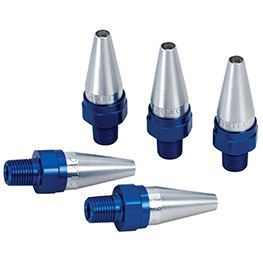
\includegraphics[width=0.5\textwidth]{nozzle.jpeg}
			\end{center}
			\caption{Boquillas de aire utilizadas en la industria.}
		\end{figure}
	\item Turbinas y compresores:
		Las \textbf{turbinas} son dispositivos capaces de convertir la energía cinética de un fluido a energía mecánica. Por otro lado, los \textbf{compresores} son dispositivos utilizados para aumentar la presión de un fluido. A los compresores se les suministra trabajo desde una fuente externa. En este sentido, podemos pensar en un compresor como un ventilador o una bomba, sin embargo tienen pequeñas diferencias que cambian su funcionalidad. Un ventilador incrementa incrementa la presión de un gas y es utilizado para movilizar el fluido. Un compresor es capaz de comprimir un gas a altar presiones. Por último, una bomba funciona igual que un compresor, sin embargo la bomba trabaja con líquidos.
		
	Características generales:
	\begin{itemize}
		\item La transferencia de calor de las turbinas es despreciable dado que están usualmente bien aisladas ($\dot Q \approx 0$). En el caso de los compresores tambien es despreciable a menos que haya enfriamiento intencional.
		\item Al igual que la transferencia de calor, el cambio en energía potencial es despreciado ($\Delta pe \cong 0$)
		\item Las velocidades en estos dispositivos, a excepción de las turbinas y ventiladores, son por lo general lo suficientemente bajas como para considerar un cambio significativo en la energía cinética ($\Delta ke \cong 0$). La velocidad de los fluidos en una turbina son muy altas, lo cual hace que el fluido experimente un cambio significativo en la energía cinética, sin ebargo este cambio es muy pequeño a comparación del cambio en entalpía del fluido.
	\end{itemize}
		\begin{figure}
			\begin{center}
			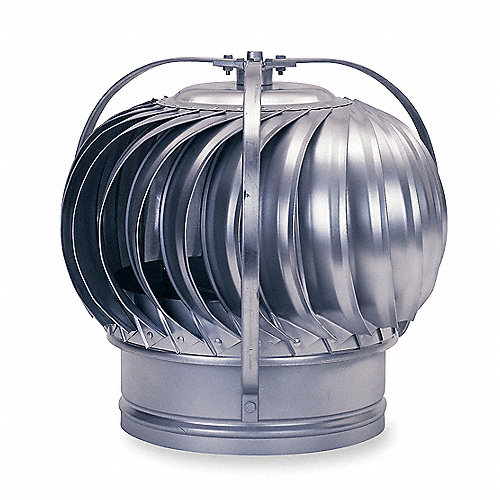
\includegraphics[width=0.5\textwidth]{turbine.jpeg}
			\end{center}
			\caption{Ventilador de turbina}
		\end{figure}
	\item Válvulas de estrangulamiento:
		Las válulas de estrangulamiento son un tipo de dispositivo que restringe el flujo del fluido en cuestión, lo que ocasiona un decremento en la presión del fluido. Lo que las diferencia de las turbinas es que estas válvulas no utilizan trabajo para hacer que la presión disminuya. La disminución en presión está acompañado de una disminución en la temperatura del fluido. Es por esta razón que las válvulas de estrangulamiento son comúnmente usadas en refrigeraciones y congeladores. El cambio en temperatura durante este proceso está gobernado por una propiedad llamada  Lo que las diferencia de las turbinas es que estas válvulas no utilizan trabajo para hacer que la presión disminuya. La disminución en presión está acompañado de una disminución en la temperatura del fluido. Es por esta razón que las válvulas de estrangulamiento son comúnmente usadas en refrigeraciones y congeladores. El cambio de temperatura en este proceso está gobernado por una propiedad llamada \textit{coeficiente de Joule-Thomson}.
	
	Características generales:
	\begin{itemize}
		\item Dado que las válvulas de estrangulamiento son por lo regular muy pequeñas es posible asumir que el flujo en ellas es adiabático ($q \cong 0$) porque no existe la suficiente área superficial para una transferencia de energía apropiada.
		\item No se ejerce ningún trabajo en el sistema ($W = 0$)
		\item El cambio en energía potencial es pequeño, despreciable. ($\Delta pe \cong 0$)
		\item A pesar de que la velocidad de salida del fluido es considerablemente más alta a la de la salida, el cambio en energía cinética es insignificante ($\Delta ke \cong 0$)
		\item La ecuación de la conservación de la energía para este dispositivo se reduce a
			\begin{align}
			h_2 \cong h_1
			\end{align}
			\begin{align}
			u_2 + P_2 V_2 \cong u_1 + P_1 V_2
			\end{align}
			esto significa que el valor de la entalpía al inicio y al final del dispositivo es el mismo. Por este motivo a las válvulas de estrangulamiento también se les conoce como \textit{dispositivos isoentálpicos}.
		\begin{figure}
			\begin{center}
			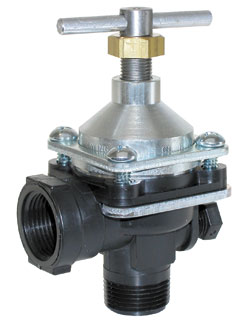
\includegraphics[width=0.3\textwidth]{tvalve.jpg}
			\end{center}
			\caption{Válvula de estrangulamiento}
		\end{figure}
	\end{itemize}
\item Cámara de mezclado: La mezcla de fluidos en ingeniería es una práctica común. El lugar donde se lleva a cabo la mezcla se le llama \textit{cámara de mezclado}. Ésta puede tomar distintas formas, entre las cuales las más poopulares son las tuberías en forma de "T" o de "Y", utilizadas comúnmente en las regaderas. El principio de conservación de la masa requiere que el flujo másico de los fluidos que entran a la cámara sea el mismo que aquél que sale de la cámara como mezcla.
	
	Características generales:
	\begin{itemize}
		\item Las cámaras de mezcla están por lo regular bien aisladas ($q \cong 0$).
		\item Usualmente no involucran algún tipo de trabajo ($W = 0$).
		\item También la energía cinética y potencial del fluido son despreciables ($ke \cong 0, pe \cong 0$).
		\item Dado que lo único por cuantificar en la ecuación de energía son las energías totales de los flujos que entran y el flujo que sale del sistema, el principio de conservación de la energía requiere que estos dos sean iguales, por lo tanto la ecuación de la conservación de la energía se vuelve análoga a la de la conservación de la masa para este caso en particular.
	\end{itemize}
		\begin{figure}
			\begin{center}
			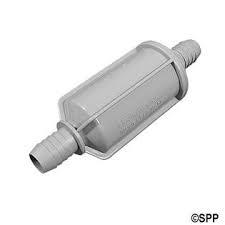
\includegraphics[width=0.3\textwidth]{mixingchamber.jpeg}
			\end{center}
			\caption{Cámara de mezclado.}
		\end{figure}
\item Intercambiador de calor: Los intercambiadores de calor son dispositivos utilizados para, como su nombre lo dice, intercambiar el calor de un fluido a otro, evitando que éstos se mezclen. Las cámaras de mezclaa veces son clasificadas como intercambiadores de calor de \textit{contacto direct}.
	Características generales:
		\begin{itemize}
			\item Los intercambiadores de calor no presentan interacción de trabajo ($W = 0$).
			\item El cambio en  energía cinética y potencial son despreciadas ($\Delta ke \cong 0, \Delta pe \cong 0$).
			\item Los intercabiadores de calor están diseñados para que exista transferencia de calor \textit{dentro} del dispositivo. Cuando todo el dispositivo es elegido como sistema para análisis, la tasa de intercabio de calor se volverá cero ($\dot Q = 0$), debido a que las fronteras del sistema estarán en donde se encuentra el aislante del dispositivo, donde ocurre poco o nada de intercambio de calor. Sin embargo, si se selecciona a un fluido como el sistema a analizar entonces existirá un intercambio de calor en el sistema diferente de cero ($\dot Q \neq 0$).
		\end{itemize}
\end{enumerate}.
		\begin{figure}
			\begin{center}
			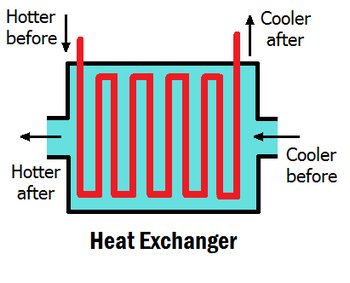
\includegraphics[width=0.5\textwidth]{heat.png}
			\end{center}
			\caption{Funcionamiento de un intercambiador de calor.}
		\end{figure}
%%%%%  Bib
\renewcommand\refname{Referencias}
\printbibliography
\end{document}
